\title{Study Guide for PHYS135B - Midterm 1}
\author{Dr. Jordan Hanson - Whittier College Dept. of Physics and Astronomy}
\date{\today}
\documentclass[10pt]{article}
\usepackage[a4paper, total={18cm, 27cm}]{geometry}
\usepackage{outlines}
\usepackage{graphicx}
\begin{document}
\maketitle

\section{Electric Charge and Electric Fields}

\begin{enumerate}
\item (a) Two charges exert $F_{\rm C} = 5.00$ N of force on each other. What will $F_{\rm C}$ be if the distance between them triples? (b) If one charge is $1$ nC, and the other is $2$ nC, what is the distance between them if $F_{\rm C} = 5.00$ N? \\ \vspace{1cm}
\item 
\begin{figure}[ht]
\centering
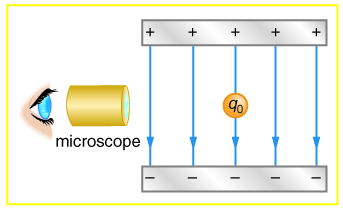
\includegraphics[width=0.3\textwidth]{figures/mill.jpeg}
\caption{\label{fig:mill} The classic Millikan oil drop experiment was a measurement of the charge of an electron.}
\end{figure}
The classic Millikan oil drop experiment was the first to measure accurately the electron charge. Oil drops were suspended against the gravitational force by a vertical electric field. (See Fig. \ref{fig:mill}.) The drops have radius $1.0 \mu$m, and a density of 920 kg/m$^3$. (a) Find the weight of the drop. (b) If the drop has a single excess electron, find the electric field strength needed to balance its weight. \\ \vspace{1.75cm}
\end{enumerate}

\section{Potential Energy and Voltage}

\begin{enumerate}
\item What is the electric field across an 10.00 nm thick human nerve cell membrane if (a) the voltage across it is 50 mV? You may assume a uniform electric field. (b) Suppose this cell membrane is part of a nerve cell.  How much energy would an electron gain if dropped through the 50 mV voltage and accelerated across the cell freely?  Express your anser in electron-Volts (eV). \\ \vspace{2cm}
\item Suppose a parallel plate capacitor is formed from a positive plate and a negative plate of charge.  The plates' areas $A$ are the same, and the plates' charges ($\pm Q$), and charge densities ($\pm Q/A = \pm \sigma$) are the same as well. (a) Write the expression for the electric field between the plates. (b) Suppose $Q = 1$ nC, and $A = 10$ mm$^2$.  What is the value of the electric field between the plates?  (c) Suppose 0 volts corresponds to the location of the negative plate.  Draw the voltage as a function of distance between the plates.  (d) What is the voltage halfway between the plates, if the plates are are separated by a distance $d = 1$ mm? \\ \vspace{2cm}
\end{enumerate}

\section{Capacitors}

\begin{enumerate}
\item What is the capacitance of the capacitor in the previous problem? \\ \vspace{1cm}
\item (a) Consider the same capacitor again, and suppose a second identical capacitor is connected \textit{in parallel} with it.  What is the total capacitance? (b) How much charge would the pair of capacitors store if the voltage across them was 5 volts? \\ \vspace{1.5cm}
\item How much energy in Joules would this charge have if it was all put to work? \\ \vspace{1cm}
\end{enumerate}

\section{Current, Resistance, and DC Circuits}

\begin{enumerate}

\item Three identical resistors $R$ are connected \textit{in parallel}, and powered by an adjustable voltage source. The voltage and \textit{total current} measurements are shown below. Determine the value of $R$.

\begin{figure}[hb]
\centering
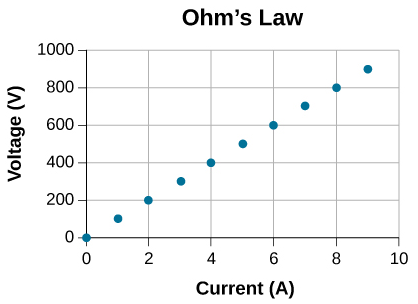
\includegraphics[width=0.33\textwidth]{figures/ohm1.png}
\caption{\label{fig:ohm1} A graph of voltage versus current.}
\end{figure}

\vspace{1cm}
\item (a) Using the PHeT tool for DC circuit construction, design a circuit in which a battery with \textit{fixed voltage} lights a bulb, but the bulb brightness can be dimmed or brightened.  \textit{Hint: use other components in series with the bulb.} Draw your design below. (b) Now make a parallel circuit in which two bulbs can be brightened or dimmed independently, and use switches to turn them on or off independently.  Draw your design below. \\ \vspace{3cm}

\clearpage

\item Figure \ref{fig:ohm2} shows a combination of series and parallel resistors and a battery. (a) Find the total resistance. (b) What is the IR voltage decrease in $R_1$? (c) Find the current $I_2$ through $R_2$. (d) What power is dissipated by $R_2$?

\begin{figure}
\centering
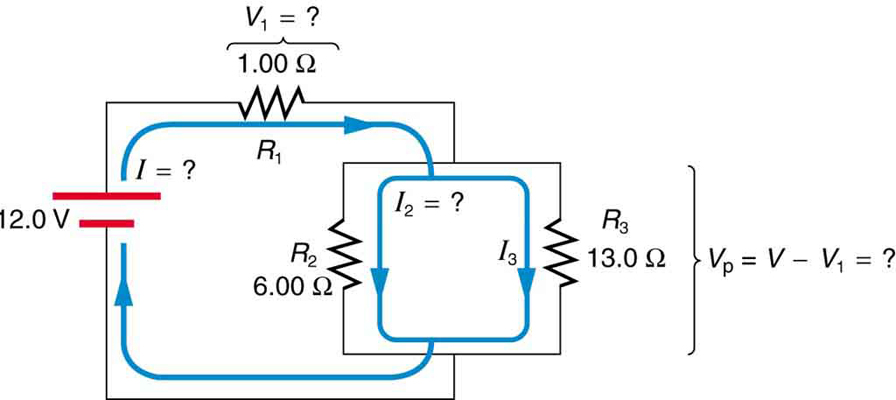
\includegraphics[width=0.5\textwidth]{figures/circuit.jpeg}
\caption{\label{fig:ohm2} A DC circuit with three resistors.}
\end{figure}
\end{enumerate}

\section{Magnetostatics I}

\begin{enumerate}
\item A proton moves at $7.50\times 10^7$ m/s perpendicular to a magnetic field. The field causes the proton to travel in a circular path of radius 0.800 m. What is the field strength? \\ \vspace{1cm}
\item (a) An oxygen-16 ion with a mass of $2.66\times10^{−26}$ kg travels at $5.00\times 10^6$ m/s perpendicular to a 1.20-T magnetic field, which makes it move in a circular arc with a 0.231-m radius. What positive charge is on the ion? (b) What is the ratio of this charge to the charge of an electron? (c) Discuss why the ratio found in (b) should be an integer. \\ \vspace{1.5cm}
\item Suppose we are designing an electric motor.  (a) What is the maximum torque on a 150-turn square loop of wire 18.0 cm on a side that carries a 50.0-A current in a 1.60-T field? (b) What is the torque when the loop makes an angle of 10.9 degrees with the field? \\ \vspace{1.5cm}
\item Nonnuclear submarines use batteries for power when submerged. (a) Find the magnetic field 50.0 cm from a straight wire carrying 1200 A from the batteries to the drive mechanism of a submarine. (b) What is the field if the wires to and from the drive mechanism are side by side? (c) Discuss the effects this could have for a compass on the submarine that is not shielded. \\ \vspace{1.5cm}
\item (a) How strong is the magnetic field inside a solenoid with 10,000 turns per meter that carries 20.0 A? (b) What current would be required to produce a B-field in this solenoid $10^4$ times a typical value of Earth's B-field?
\end{enumerate}

\end{document}